% This is part of (everything) I know in mathematics
% Copyright (c) 2011-2013,2016-2018
%   Laurent Claessens
% See the file fdl-1.3.txt for copying conditions.

%+++++++++++++++++++++++++++++++++++++++++++++++++++++++++++++++++++++++++++++++++++++++++++++++++++++++++++++++++++++++++++
\section{Isométries de l'espace euclidien}
%+++++++++++++++++++++++++++++++++++++++++++++++++++++++++++++++++++++++++++++++++++++++++++++++++++++++++++++++++++++++++++

Nous considérons l'espace affine euclidien \( A=\affE_n(\eR)\) modelé sur \( \eR^n\) avec sa métrique usuelle. Un premier grand résultat sera le théorème \ref{ThoDsFErq} qui dira que les isométries de cet espace sont des applications linéaires.

%--------------------------------------------------------------------------------------------------------------------------- 
\subsection{Structure du groupe  \texorpdfstring{\( \Isom(\eR^n)\)}{Isom(Rn)} }
%---------------------------------------------------------------------------------------------------------------------------

\begin{example}
    La forme quadratique \( q(x)=x_1^2+x_2^2\) donne la norme euclidienne. La forme bilinéaire associée est \( b(x,y)=x_1y_1+x_2y_2\), qui est le produit scalaire usuel.
\end{example}

Il ne faudrait pas déduire trop vite que la formule \( \| x \|^2=q(x)\) donne une norme dès que \( q\) est non dégénérée. En effet \( q\) peut ne pas être définie positive. La forme \( q(x)=x_1^2-x_2^2\) prend des valeurs positives et négatives. A fortiori \( d(x,y)=q(x-y)\) ne donne pas toujours une distance.

\begin{definition}      \label{DEFooECTUooRxBhHf}
    Une \defe{isométrie}{isométrie!de forme quadratique} pour la forme quadratique \( q\) est une application bijective \( f\colon V\to V\) telle que \( q(x-y)=q\big( f(x)-f(y) \big)\). Dans les cas où \( q\) donne une distance, alors c'est une isométrie au sens usuel.
\end{definition}

\begin{lemma}   \label{LemewGJmM}
    Soient \( q\) une forme quadratique et \( b\) la forme bilinéaire associée par le lemme \ref{LEMooLKNTooSfLSHt}.  Pour une application bijective \( f\colon E\to E\) telle que \( f(0)=0\), les conditions suivantes sont équivalentes: 
    \begin{enumerate}
        \item
            \( b\big( f(x),f(y) \big)=b(x,y)\) pour tout \( x,y\in E\);
        \item
            \( q\big( f(x)-f(y) \big)=q(x-y)\) pour tout \( x,y\in E\).
    \end{enumerate}
\end{lemma}

\begin{proof}
    Dans le sens direct, en posant \( x=y\) nous trouvons tout de suite \( q(f(x))=q(f)\); ensuite en utilisant la distributivité de \( b\),
    \begin{subequations}
        \begin{align}
            q\big( f(x)-f(y) \big)&=b\big( f(x)-f(y),f(x)-f(y) \big)\\
            &=q\big( f(x) \big)-2b\big( f(x),f(y) \big)+q\big( f(y) \big)\\
            &=q(x)+q(y)-2b(x,y)\\
            &=q(x-y).
        \end{align}
    \end{subequations}
    
    Dans l'autre sens, nous commençons par remarquer que l'hypothèse \( f(0)=0\) donne \( q(x)=q\big( f(x) \big)\). Ensuite nous utilisons l'identité de polarisation \eqref{EqMrbsop} :
    \begin{subequations}
        \begin{align}
            b\big( f(x),f(y) \big)&=\frac{ 1 }{2}\big[ q\big( f(x) \big)+q\big( f(y) \big)-q\big( f(x-y) \big) \big]\\
            &=\frac{ 1 }{2}\big[ q(x)+q(y)-q(x-y) \big]\\
            &=b(x,y).
        \end{align}
    \end{subequations}
\end{proof}

\begin{theorem}[\cite{ooQFKAooFnllQU}]     \label{ThoDsFErq}
    Soit \( f\colon E\to E\) une bijection telle que
    \begin{equation}
        q(x-y)=q\big( f(x)-f(y) \big)
    \end{equation}
    pour tout \( x,y\in E\). Alors
    \begin{enumerate}
        \item
            si \( f(0)=0\), alors \( f\) est linéaire;
        \item
            si \( f(0)\neq 0\) alors \( f\) est affine\footnote{Lemme \ref{LEMooZZAIooOMiayy}.}
    \end{enumerate}
\end{theorem}

\begin{proof}
    Si \( f(0)=0\), nous savons par le lemme \ref{LemewGJmM} que \( b\big( f(x),f(y) \big)=b(x,y)\). Soit \( z\in E\); étant donné que \( f\) est bijective nous pouvons considérer l'élément \( f^{-1}(z)\in E\) et calculer
    \begin{subequations}
        \begin{align}
            b\big( f(x+y),z \big)&=b\big( f(x+y),f(f^{-1}(z)) \big)\\
            &=b(x+y,f^{-1}(z))\\
            &=b(x,f^{-1}(z))+b(y,f^{-1}(z))\\
            &=b(f(x),z)+b(f(y),z)\\
            &=b\big( f(x)+f(y),z \big),
        \end{align}
    \end{subequations}
    donc \( f(x+y)=f(x)+f(y)\) par le lemme \ref{LemyKJpVP}. 

    De la même façon on trouve \( b\big( f(\lambda x),z \big)=b\big( \lambda f(x),z \big)\) qui prouve que \( f(\lambda x)=\lambda f(x)\) et donc que \( f\) est linéaire.

    Si \( f(0)\neq 0\), alors nous posons \( g(x)=f(x)-f(0)\) qui vérifie \( g(0)=0\) et
    \begin{equation}
        q\big( g(x)-g(y) \big)=q\big( f(x)-f(0)-f(y)+f(0) \big)=q(x-y).
    \end{equation}
    Nous pouvons donc appliquer le premier point à \( g\), déduire que \( g\) est linéaire et donc que \( f\) est affine.
\end{proof}

\ifbool{isEverything}{
\begin{remark}
    Des preuves alternatives.
    \begin{enumerate}
        \item
            En utilisant un peut plus d'indices et un peu plus de mots comme «tenseurs», peut être trouvée  \href{http://physics.stackexchange.com/questions/12664/proving-that-interval-preserving-transformations-are-linear}{ici}. Le fait que la preuve donnée soit tensorielle me fait penser que le résultat peut encore être généralisé.
        \item
            Et encore une autre preuve, utilisant des techniques de groupes de Lie sera la proposition \ref{PROPooDVIWooAFDNPy}.
    \end{enumerate}
\end{remark}
}
{}

Nous pouvons maintenant particulariser tout cela au cas de \( \eR^n\) muni du produit scalaire usuel et de la norme associée pour voir quel résultat nous avons à peine prouvé.

\begin{lemma}[\cite{ooYPVPooYGSlNU}]        \label{LEMooJPYZooHETCqt}
    Une isométrie est bijective (nous sommes en dimension finie).
\end{lemma}

\begin{proof}
    Si \( f\colon E\to E\) est une isométrie, elle est linéaire par le théorème \ref{ThoDsFErq}. Elle vérifie également \( \| f(x) \|=\| x \|\), et donc \( f(x)=0\) si et seulement si \( x=0\), c'est à dire que \( f\) est injective. Elle est alors bijective par le corollaire \ref{CORooCCXHooALmxKk} du théorème du rang.
\end{proof}

Nous notons ici \( T(n)\) le groupe des translations sur \( \eR^n\). Un élément de \( T(n)\) est une translation \( \tau_v\) donnée par un vecteur \( v\) et agissant sur \( \eR^n\) par
\begin{equation}
    \begin{aligned}
        \tau_v\colon \eR^n&\to \eR^{n} \\
        x&\mapsto x+v. 
    \end{aligned}
\end{equation}
Ce groupe est isomorphe au groupe abélien \( (\eR^n,+)\), et nous allons souvent identifier \( \tau_v\) à \( v\).

Si vous ne voulez pas savoir ce qu'est un produit semi-direct de groupes, vous pouvez lire seulement le point \ref{ITEMooLLUIooIGsknv} du théorème suivant, et passer directement à la remarque \ref{REMooLUEZooIwvTqu}.
\begin{theorem}     \label{THOooQJSRooMrqQct}
    Un peu de structure sur \( \Isom(\eR^n)\).
    \begin{enumerate}
        \item       \label{ITEMooLLUIooIGsknv}
            L'application
            \begin{equation}
                \begin{aligned}
                    \psi\colon T(n)\times \gO(n)&\to \Isom(\eR^n) \\
                    (v,\Lambda)&\mapsto \tau_v\circ\Lambda 
                \end{aligned}
            \end{equation}
            est une bijection. Ici,  \( T(n)\) est le groupe des translations de \( \eR^n\).
        \item
            Un couple \( (v,\Lambda)\in T(n)\times\SO(n)\) agit sur \( x\in \eR^n\) par
            \begin{equation}
                (v,\Lambda)x=\Lambda x+v
            \end{equation}
            au sens où \( \psi(v,\Lambda)x=\Lambda x+v\).
        \item       \label{ITEMooEWSIooNKzRxB}
            En tant que groupes,
            \begin{equation}
                \Isom(\eR^n)\simeq T(n)\times_{\rho}\gO(n)
            \end{equation}
            où \( \rho\) représente l'action adjointe de \( \gO(n)\) sur \( T(n)\) et \( \times_{\rho}\) dénotes le produit semi-direct de la définition \ref{DEFooKWEHooISNQzi}.
    \end{enumerate}
\end{theorem}

\begin{proof}
    Point par point.
    \begin{enumerate}
        \item
            Prouvons que l'application proposée est injective et surjective. Notons aussi que ce point ne parle pas de structure de groupe, mais seulement d'une bijection en tant qu'ensembles.    
            \begin{subproof}
                \item[Injection]
                    Si \( \psi(v,\Lambda)=\psi(w,\Lambda')\) alors en appliquant sur \( x=0\) nous avons tout de suite \( v=w\). Et ensuite \( \Lambda=\Lambda'\) est immédiat.
                \item[Surjection]
                    Une isométrie \( g\in\Isom(\eR^n)\) est une application \( g\colon \eR^n\to \eR^n\) telle que \( d(x,y)=d\big( g(x),g(y) \big)\). Dans le cas de \( \eR^n\) cela se traduit par
                    \begin{equation}
                        \| x-y \|=\big\| g(x)-g(y) \big\|,
                    \end{equation}
                    Vu que \( x\mapsto\| x \|\) est une forme quadratique, elle tombe sous le coup du théorème  \ref{ThoDsFErq}, ce qui nous permet de dire que \( g\) est affine. Or par définition une application est affine lorsqu'elle est la composée d'une translation et d'une application linéaire.
            \end{subproof}
        \item
            C'est seulement le fait que \( (\tau_v\circ\Lambda)x=\tau_v\big( \Lambda x \big)=\Lambda(x)+v\).
        \item
            Nous allons étudier l'application
            \begin{equation}
                \psi\colon T(n)\times_{\rho}O(n)\to \Isom(\eR^n).
            \end{equation}
            \begin{subproof}
            \item[Le produit semi-direct est bien définit]
                Il faut montrer que
                \begin{equation}
                    \begin{aligned}
                        \rho\colon O(n)&\to \Aut\big( T(n) \big) \\
                        \Lambda&\mapsto \AD(\Lambda) 
                    \end{aligned}
                \end{equation}
                est correcte.

                D'abord pour \( \Lambda\in O(n)\), nous avons bien \( \rho_{\Lambda}(\tau_v)\in T(n)\) parce qu'en appliquant à \( x\in \eR^n\),
                    \begin{equation}
                        (\Lambda\tau_v\Lambda^{-1})(x)=\Lambda\big( \tau_v(\Lambda^{-1} x) \big)=\Lambda\big( \Lambda^{-1}x+v \big)=x+\Lambda(v)=\tau_{\Lambda(v)}(x).
                    \end{equation}
                    Donc \( \rho_{\Lambda}(\tau_v)=\tau_{\Lambda(v)}\).

                    De plus, \( \rho_{\Lambda}\in\Aut\big( T(n) \big)\) parce que 
                    \begin{equation}
                        \rho_{\Lambda}\big( \tau_v\circ \tau_w \big)=\rho_{\Lambda}(\tau_v)\circ\rho_{\Lambda}(\tau_v),
                    \end{equation}
                    comme on peut aisément vérifier que les deux membres sont égaux à \( \tau_{\Lambda(v+w)}\).
                \item[\( \psi\) est une bijection]
                    Cela est déjà vérifié.
                \item[\( \psi\) est un homomorphisme]
                    Nous avons d'une part
                    \begin{equation}
                        \psi\big( (v,g)(w,h) \big)=\psi\big( v\rho_g(w),gh \big)=\tau_v\circ g\circ\tau_w\circ g^{-1}\circ g\circ h=\tau_v\circ g\circ\tau_w\circ h.
                    \end{equation}
                    Et d'autre part,
                    \begin{equation}
                        \psi(v,g)\circ\psi(w,h)=\tau_v\circ g\circ \tau_w\circ h,
                    \end{equation}
                    ce qui est la même chose.
            \end{subproof}
    \end{enumerate}
\end{proof}

\begin{remark}      \label{REMooLUEZooIwvTqu}
    Notons au passage la loi de groupe sur les couples qui est donnée, pour tout \( v,v'\in \eR^n\), \( \Lambda,\Lambda'\in\SO(n)\), par
    \begin{equation}    \label{EqDiHcut}
            (v,\Lambda)\cdot(v',\Lambda')=(\Lambda v'+v,\Lambda\Lambda')
    \end{equation}
    comme le montre le calcul suivant :
    \begin{subequations}
        \begin{align}
            (v,\Lambda)\cdot(v',\Lambda')x&=(v,\Lambda)(\Lambda'x+v')\\
            &=\Lambda\Lambda'x+\Lambda v'+v\\
            &=(\Lambda v'+v,\Lambda\Lambda')x.
        \end{align}
    \end{subequations}
\end{remark}

\begin{proposition}[\cite{ooZYLAooXwWjLa}]      \label{PROPooDHYWooXxEXvl}
    Soient \( n\geq 1\) et \( R\) un élément de \( \gO(n)\) de déterminant \( -1\) tels que \( R^2=\id\). En posant \( C_2=\{ \id,R \}\) nous avons
    \begin{equation}
        \gO(n)=\SO(n)\times_{\rho} C_2
    \end{equation}
\end{proposition}

\begin{proof}
    Notons que pour \( R\) nous pouvons prendre par exemple \( (x_1,\ldots, x_n)\mapsto (-x_1,x_2,\ldots, x_n)\). Ce que nous allons montrer être un isomorphisme est :
    \begin{equation}
        \begin{aligned}
            \psi\colon \SO(n)\times C_2&\to \gO(n) \\
            (A,h)&\mapsto Ah. 
        \end{aligned}
    \end{equation}
    \begin{subproof}
        \item[Injectif]
            Soient \( A,B\in \SO(n)\) et \( h,k\in C_2\) tels que \( \psi(A,h)=\psi(B,k)\), c'est à dire tels que \( Ah=Bk\). Vu que \( \det(A)=\det(B)=1\) nous avons \( \det(h)=\det(k)\). Mais comme \( C_2\) contient un élément de déterminant \( 1\) et un élément de déterminant \( -1\), nous avons \( h=k\). De là \( A=B\).
        \item[Surjectif]
            Soit \( X\in\gO(n)\). Si \( \det(X)=1\) alors \( X\in \SO(n)\) et \( X=\psi(X,\mtu)\). Si par contre \( \det(X)=-1\) alors \( XR\in\SO(n)\) parce que \( \det(XR)=1\) et nous avons
            \begin{equation}
                \psi(XR,R)=XR^2=X.
            \end{equation}
        \item[Homomorphisme]
            Nous avons
            \begin{equation}
                \psi\Big( (A,h)(B,k) \Big)=\psi\big( A\rho_h(B),hk \big)=A(hBh^{-1})hk=AhBk,
            \end{equation}
            tandis que
            \begin{equation}
                \psi(A,h)\psi(B,k)=AhBk,
            \end{equation}
            qui est la même chose.
    \end{subproof}
\end{proof}

\begin{lemma}[\cite{JGAdTA}]
    Si \( n\geq 3\), alors toute droite est intersection de deux plans non isotropes.
\end{lemma}

\begin{proposition}[\cite{ooZYLAooXwWjLa}]      \label{PROPooVEEUooJQmmkN}
    Si une isométrie de \( \eR^n\) fixe un ensemble \( F\) de points, alors elle fixe l'espace affine engendrée par \( F\).
\end{proposition}

\begin{proof}
    Soit \( f\in \Isom(\eR^n)\) fixant \( F\). Par le théorème \ref{ThoDsFErq}, c'est une application affine et l'ensemble \( \Fix(f)\) des points fixés par \( f\) est un sous-espace affine de \( \eR^n\), grâce à la proposition \ref{PROPooYRCJooIcmUVI}.

    Donc \( \Fix(f)\) est un espace affine contenant \( F\). Vu que l'espace affine engendré par \( F\) est l'intersection de tous les espaces affines contenant \( F\), il est en particulier contenu dans \( \Fix(f)\).
\end{proof}

\begin{corollary}       \label{CORooZHZZooDgTzsW}
    Si \( f\) et \( g\) sont des isométries de \( \eR^n\) qui coïncident sur \( F\), alors elles coïncident sur l'espace affine engendré par \( F\).
\end{corollary}

\begin{proof}
    Nous considérons \( h=g^{-1}\circ f\) qui est une isométrie de \( \eR^n\) fixant \( F\). Elle fixe donc, par la proposition \ref{PROPooVEEUooJQmmkN}, l'espace affine engendré par $F$. Or tout point fixé par \( h\) est un point sur lequel \( g\) et \( f\) coïncident.
\end{proof}

%--------------------------------------------------------------------------------------------------------------------------- 
\subsection{Classification des isométries de \( \eR\)}
%---------------------------------------------------------------------------------------------------------------------------

\begin{definition}
    Soit \( x\in \eR\); nous notons \( \sigma_x\) la \defe{réflexion}{réflexion}\nomenclature[R]{\( \sigma_x\)}{réflexion par rapport à \( x\)} par rapport à \( x\), c'est à dire
    \begin{equation}
        \sigma_x(y)=2x-y.
    \end{equation}
\end{definition}

\begin{theorem}[\cite{ooZYLAooXwWjLa}]
    Toute isométrie de \( \eR\) est composée d'au plus \( 2\) réflexions. Plus précisément toute isométrie de \( \eR\) est dans une des trois catégories suivantes :
    \begin{itemize}
        \item l'identité (\( 0\) réflexions),
        \item les réflexions,
        \item les translations (\( 2\) réflexions)
    \end{itemize}
\end{theorem}

\begin{proof}
    Nous divisions la preuve en fonction du nombre de points fixés par l'isométrie \( f\in\Isom(\eR)\).
    \begin{subproof}
        \item[\( f\) fixe deux points distincts]
            Alors elle fixe l'espace affine engendrée par ces deux points par la proposition \ref{PROPooVEEUooJQmmkN}. Donc \( f\) fixe tout \( \eR\) et est l'identité.
        \item[\( f\) fixe un unique point]
            Soit \( x\) l'unique point fixé par \( f\) et considérons \( y\neq x\). Vu que \( x=f(x)\) et que \( f\) est une isométrie,
            \begin{equation}
                d\big( x,f(y) \big)=d\big( f(x),f(y) \big)=d(x,y).
            \end{equation}
            Donc \( f(y)\) est à égale distance de \( x\) que \( y\). Autrement dit, \( f(y)\) est soit \( y\) soit \( \sigma_x(y)\). Mais comme \( x\) est unique point fixe, \( f(y)=\sigma_x(y)\). Ce raisonnement étant valable pour tout \( y\neq x  \) nous avons \( f=\sigma_x\).
        \item[\( f\) n'a pas de points fixes]
            Soient \( x\in \eR\) et \( y=\frac{ x+f(x) }{ 2 }\). Nous posons \( g=\sigma_y\circ f\). Alors \( x\) est un point fixe de \( g\) parce que
            \begin{equation}
                g(x)=\sigma_y\big( f(x) \big)=2y-f(x)=x.
            \end{equation}
            Donc soit \( g\) est l'identité soit \( g\) est une réflexion (par les points précédents). La possibilité \( g=\id\) est exclue parce que cela ferait \( f=\sigma_y\) alors que \( f\) n'a pas de points fixes. Donc \( g\) est une réflexion; et comme \( x\) est un point fixe de \( g\) nous avons \( g=\sigma_x\). Au final
            \begin{equation}
                f=\sigma_y\circ\sigma_x.
            \end{equation}
            Montrons que cela implique que \( f\) est une translation :
            \begin{equation}
                \sigma_y\sigma_x(z)=\sigma_y(2x-z)=2y-2x+z=z+2(y-x).
            \end{equation}
            Donc \( \sigma_y\circ\sigma_x\) est la translation de vecteur \( 2(y-x)\).
    \end{subproof}
\end{proof}


%--------------------------------------------------------------------------------------------------------------------------- 
\subsection{Segment, plan médiateur et équidistance}
%---------------------------------------------------------------------------------------------------------------------------

\begin{lemma}   \label{LEMooSZZWooPDHnGl}
    Un point \( M\) est sur la médiatrice du segment \( [A,B]\) si et seulement si \( \| M-A \|=\| M-B \|\).
\end{lemma}

\begin{lemma}       \label{LEMooVBVUooOTFFXT}
    Soient \( A\) et \( B\) de points de \( \eR^3\). Alors le plan médiateur du segment \( [A,B]\) est le lieu des points de \( \eR^3\) à être équidistants de \( A\) et \( B\).
\end{lemma}

\begin{proof}
    Nous nommons \( \sigma\) ce plan.

    Soit \( X\) un point équidistant de \( A\) et \( B\). Alors dans le plan \( (A,B,X)\), le triangle \( ABX\) est isocèle en \( X\), et la hauteur issue de \( X\) coupe perpendiculairement \( [A,B]\) en son milieu. Cela prouve que \( X\) est dans le plan médiateur du segment \( [A,B]\) (lemme \ref{LEMooSZZWooPDHnGl}).

    Mettons au contraire que \( X\) est dans le plan médiateur de \( [A,B]\). Nous avons \( (X,M)\perp (A,B)\). Donc le triangle \( A,B,X\) est isocèle en \( X\) et donc \( X\) est équidistant de \( A\) et \( B\).
\end{proof}

%--------------------------------------------------------------------------------------------------------------------------- 
\subsection{Isométries du tétraèdre régulier}
%---------------------------------------------------------------------------------------------------------------------------

\begin{definition}
    Un polyèdre \defe{régulier}{régulier!polyèdre} est un polyèdre dont les faces sont des polygones réguliers identiques dont tous les sommets joignent le même nombre d'arrêtes.
\end{definition}

Le \defe{tétraèdre}{tétraèdre} est une pyramide à base triangulaire dont toutes les faces sont des triangles équilatéraux.

\begin{proposition}[Isométries affines du tétraèdre régulier]       \label{PROPooVNLKooOjQzCj}
    Soient \( T\) un tétraèdre régulier et \( \Iso(T)\) son groupe d'isométries affines (définition \ref{DEFooZGKBooGgjkgs}). Alors
    \begin{equation}
        \Iso(T)\simeq S_4
    \end{equation}
    où \( S_4\) est le groupe des permutations de quatre objets.
\end{proposition}

\begin{proof}
    Commençons par prouver qu'une isométrie préserve les sommets : l'image d'un sommet est un sommet. Pour cela nous considérons \( g\in \Iso(T)\) et nous supposons que l'image d'un sommet \( x\) soit à l'intérieur d'une arrête. Soient \( g(y)\) et \( g(z)\) deux points distincts de cette arrête situés à égale distance de \( g(x)\). Cela est possible parce que \( g\) est une bijection de \( \eR^3\). Aussi : \( y\neq z\). Mais une application affine préserve l'alignement (vous ne le croyez pas  ? regardez la forme donnée par le lemme \eqref{LEMooZZAIooOMiayy}), donc \( x\), \( y\) et \( z\) foment un triangle isocèle en \( x\) de points alignés et appartenant à \( T\). Cela est impossible si \( x\) est un sommet.

    Donc l'image d'un sommet est un sommet. Si nous numérotons les sommets \( x_1\),\ldots, \( x_4\), nous obtenons un morphisme de groupe \( \varphi\colon \Isom(T) \to S_4\) qui envoie \( g\) sur la permutation qui envoie \( 1\) sur le numéro du sommet \( g(x_1)\), \( 2\) sur le numéro du sommet \( g(x_2)\), etc.

    \begin{subproof}
    \item[Le morphisme \( \varphi\) est injectif]
        Supposons \( \varphi(g_1)=\varphi(g_2)\). Alors \( g_1^{-1}\circ g_2\) est une isométrie de \( (\eR^3,d)\) qui fixe les quatre sommets. Une application affine \( \eR^4\to\eR^3\) fixant \( 4\) point est l'identité par le lemme \ref{LEMooDUMVooFtfFOe}. Donc \( g_1^{-1}g_2=\id\), ce qui prouve que \( g_1=g_2\). Vous noterez que nous utilisons l'unicité de l'inverse dans un groupe.

    \item[\( \varphi\) est surjectf]

        Nous savons que \( S_4\) est engendré par les transpositions (proposition \ref{PropPWIJbu}). Or les transpositions sont dans l'image de \( \varphi\). En effet, notons les sommets de notre tétraèdre par \( A\), \( B\), \( D\) et \( D\) et considérons la transposition \( A\leftrightarrow B\). Elle est l'image par \( \varphi\) de la réflexion selon le plan \( \sigma\), médiateur du segment \( [A,B]\). Pour nous assurer de cela, nous devons nous assurer que \( C\) et \( D\) appartiennent à \( \sigma\). Cela est le contenu du lemme \ref{LEMooVBVUooOTFFXT}.

    \item[Conclusion]

        L'application \( \varphi\) est un morphisme bijectif, c'est à dire un isomorphisme.

    \end{subproof}
\end{proof}

\begin{normaltext}
    Lorsque le tétraèdre a son barycentre en l'origine de \( \eR^3\), l'isomorphisme \( \varphi\colon \Iso(T)\to S_4\) donne une représentation de dimension \( 3\) de \( S_4\). Nous allons calculer les caractères de \( S_4\) en la section \ref{SecUMIgTmO} sans avoir besoin de savoir que l'une des représentations de dimension \( 3\) est cella que nous venons de trouver via le groupe des isométries du tétraèdre. Nous allons cependant également y calculer les caractères de la représentations \( \varphi\), pour le sport.

    Plus de détails en \ref{SUBSECooLEUAooGGjGIZ}.
\end{normaltext}

%+++++++++++++++++++++++++++++++++++++++++++++++++++++++++++++++++++++++++++++++++++++++++++++++++++++++++++++++++++++++++++ 
\section{Trigonométrie}
%+++++++++++++++++++++++++++++++++++++++++++++++++++++++++++++++++++++++++++++++++++++++++++++++++++++++++++++++++++++++++++

%--------------------------------------------------------------------------------------------------------------------------- 
\subsection{Définitions, périodicité et quelque valeurs remarquables}
%---------------------------------------------------------------------------------------------------------------------------

\begin{propositionDef}[Défintion du cosinus et du sinus]        \label{PROPooZXPVooBjONka}
    La série
    \begin{equation}
        \cos(x)=\sum_{n=0}^{\infty}\frac{ (-1)^n }{ (2n)! }x^{2n}
    \end{equation}
    définit une fonction \( \cos\colon \eR\to \eR\) de classe \(  C^{\infty}\). Nous l'appelons \defe{cosinus}{cosinus}

    La série
    \begin{equation}        \label{EQooCMRFooCTtpge}
        \sin(x)=\sum_{n=0}^{\infty}\frac{ (-1)^n }{ (2n+1)! }x^{2n+1}
    \end{equation}
    définit une fonction \( \sin\colon \eR\to \eR\) de classe \(  C^{\infty}\). Nous l'appelons \defe{sinus}{sinus}
\end{propositionDef}

\begin{proof}
    La série entière définissant \( \cos(x)\) a pour coefficients
    \begin{equation}
        a_n=\begin{cases}
            0    &   \text{si } n\text{ est impair}\\
            \frac{ (-1)^{n/2} }{ n! }    &   \text{si } n\text{ est pair}.
        \end{cases}
    \end{equation}
    Nous pouvons la majorer par la série entière donnée par les coefficients
    \begin{equation}
        b_n=\begin{cases}
            1/n!    &   \text{si } n\text{ est impair}\\
            \frac{ (-1)^{n/2} }{ n! }    &   \text{si } n\text{ est pair}.
        \end{cases}
    \end{equation}
    Quelle que soit la parité de \( k\) nous avons toujours
    \begin{equation}
        | \frac{ b_{k+1} }{ b_k } |=\frac{1}{ k+1 },
    \end{equation}
    de telle sorte que la formule d'Hadamard \eqref{EqAlphaSerPuissAtern} nous donne \( R=\infty\) pour la série \( \sum_{k=0}^{\infty}b_kx^k\). A fortiori\footnote{Remarque \ref{REMooYOTEooKvxHSf}.} le rayon de convergence pour la série du cosinus est infini.

    L'assertion concernant le sinus se démontre de même.

    En ce qui concerne le fait que les fonctions \( \sin\) et \( \cos\) sont de classe \(  C^{\infty}\) sur \( \eR\), il faut invoquer le corollaire \ref{CorCBYHooQhgara}.
\end{proof}

\begin{lemma}
    En ce qui concerne la dérivation, nous avons
    \begin{subequations}
        \begin{align}
            \sin'&=\cos\\
            \cos'&=-\sin.
        \end{align}
    \end{subequations}
\end{lemma}

\begin{proof}
    Il s'agit de se permettre de dériver terme à terme (proposition \ref{ProptzOIuG}) les séries qui définissent le sinus et le cosinus.
\end{proof}

\begin{lemma}       \label{LEMooAEFPooGSgOkF}
    Les fonctions sinus et cosinus vérifient
    \begin{equation}
        \cos^2(x)+\sin^2(x)=1
    \end{equation}
    pour tout \( x\in \eR\).
\end{lemma}

\begin{proof}
    Posons \( f(x)=\sin^2(x)+\cos^2(x)\) et dérivons :
    \begin{equation}
        f'(x)=2\sin(x)\cos(x)+2\cos(x)(-)\sin(x)=0.
    \end{equation}
    La fonction \( f\) est donc constante par le corollaire \ref{CORooEOERooYprteX}. Nous avons donc pour tout \( x\) :
    \begin{equation}
        f(x)=f(0)=\sin^2(0)+\cos^2(0)=1.
    \end{equation}
    Le dernier calcul s'obtient en substituant directement \( x\) par zéro dans les séries : \( \sin(0)=0\) et \( \cos(0)=1\).
\end{proof}

\begin{lemma}       \label{LEMooHOYZooKQTsXW}
    Nous avons la formule
    \begin{equation}        \label{EQooRVPJooTMwNTU}
        e^{ix}=\cos(x)+i\sin(x)
    \end{equation}
    pour tout \( x\in \eR\).

    En particulier pour tout \( x\), nous avons \( |  e^{ix} |=1\).
\end{lemma}
Nous en dirons plus dans la proposition \ref{PROPooZEFEooEKMOPT}.

\begin{proof}
    La définition de l'exponentielle sur \( \eC\) est la définition \ref{DEFooSFDUooMNsgZY}. Cette définition fonctionne parce que \( \eC\) est une algèbre normée, et que \( \eC\) est un \( \eC\)-module vérifiant l'inégalité \(  | zz' |\leq | z | |z' | \) (en l'occurrence, une égalité).

    Nous remarquons que que \( i^k\) vaut \( 1\), \( i\), \( -1\), \( -i\). Donc un terme sur deux est imaginaire pur et parmi ceux-là, un sur deux est positif. À bien y regarder, les termes imaginaires purs forment la série du sinus et ceux réels la série du cosinus.
\end{proof}

\begin{lemma}       \label{LEMooJAWBooJGfZIL}
    Nous avons les formules d'addition d'angles
    \begin{subequations}        \label{SUBEQSooFSSMooHcYwRc}
        \begin{align}
            \cos(a+b)=\cos(a)\cos(b)-\sin(a)\sin(b) \label{EQooJYEMooQaOMib}\\
            \sin(a+b)=\cos(a)\sin(b)+\sin(a)\cos(b) \label{EQooECAUooQzckDv}\\
            \cos(a-b)=\cos(a)\cos(b)+\sin(a)\sin(b) \label{EQooCVZAooQfocya}
        \end{align}
    \end{subequations}
    pour tout \( a\), \( b\) réels.
\end{lemma}  

\begin{proof}
    Nous utilisons la formule d'addition dans l'exponentielle, proposition \eqref{EQooVFXUooBfwjJY} et la formule \eqref{EQooRVPJooTMwNTU} avant de séparer les parties réelles et imaginaires :
    \begin{equation}
        e^{i(a+b)}= e^{ia} e^{ib}=\cos(a)\cos(b)-\sin(a)\sin(b)+i\big( \cos(a)\sin(b)+\sin(a)\cos(b) \big).
    \end{equation}
    Cela est également égal à
    \begin{equation}
        \cos(a+b)+i\sin(a+b).
    \end{equation}
    En identifiant les parties réelle et imaginaires, nous obtenons les formules \eqref{EQooJYEMooQaOMib} et \eqref{EQooCVZAooQfocya} annoncées. 

    Pour la formule \eqref{EQooCVZAooQfocya}, il suffit de se souvenir que \( \sin(-b)=-\sin(b)\) et \( \cos(-b)=\cos(b)\) (ces deux égalités sont immédiatement visibles sur les développements en série : l'un a uniquement des puissances paires et l'autre impaires) et d'écrire \eqref{EQooJYEMooQaOMib} avec \( -b\) au lieu de \( b\).
\end{proof}

\begin{corollary}       \label{CORooQZDQooWjMXTF}
    Les formules suivantes pour les duplications d'angles s'ensuivent : 
    \begin{subequations}
        \begin{align}
            \cos(2a)&=\cos^2(a)-\sin^2(a)\\
            \sin(2a)&=2\cos(a)\sin(a).
        \end{align}
    \end{subequations}
\end{corollary}

\begin{proof}
    Poser \( b=a\) dans les relations du lemme \ref{LEMooJAWBooJGfZIL}.
\end{proof}

\begin{lemma}       \label{LEMooPQWWooMdPWUT}
    Un sous-groupe de \( (\eR,+)\) est soit dense dans \( \eR\) soit de la forme \( p\eZ\) pour un certain réel \( p\neq 0\).
\end{lemma}

\begin{proof}
    Soit \( A\), un sous-groupe de \( (\eR,+)\) qui ne soit pas dense. Soit un intervalle \( \mathopen] a , b \mathclose[\) qui n'intersecte pas \( A\) (si vous voulez frimer, vous noterez ici que nous utilisons le fait que les intervalles ouverts forment une base de la topologie de \( \eR\)). Si \( d=| b-a |\), l'ensemble \( A\) ne contient pas deux éléments séparés par strictement moins de \( d\). Soit \( p\), le plus petit élément strictement positif de \( A\); nous avons \( p\geq d\) (parce que \( 0\in A\) de toutes façons).

        Vu que \( A\) est un groupe nous avons \( p\eZ\subset A\).

        Pour l'inclusion inverse, si \( x\in A\) est hors de \( p\eZ\), il existe un \( y\in p\eZ\) avec \( | x-y |<p\). Et donc le nombre \( | x-y |\) est dans \( A\) tout en étant plus petit que \( p\). Contradiction.
\end{proof}

\begin{proposition}[\cite{ooUMDHooHrJpfV}]      \label{PROPooFRVCooKSgYUM}
    La fonction \( \cos\) est périodique et le nombre \( T>0\) est une période si et seulement si \( \cos(T)=1\) et \( \sin(T)=0\).
\end{proposition}

\begin{proof}
    Plusieurs étapes.
    \begin{subproof}
        \item[La fonction cosinus n'est pas toujours positive]
    Supposons d'abord que \( \cos(x)>0\) pour tout \( x\in \eR\). Dans ce cas, la fonction \( \sin\) est strictement croissante. Mais les deux fonctions sont bornées par \( 1\) du fait de la formule \( \cos^2(x)+\sin^2(x)=1\). La fonction \( \sin\) étant croissante et bornée, elle est convergente vers un réel par la proposition \ref{PropMTmBYeU} :
    \begin{equation}
        \lim_{x\to \infty} \sin(x)=\ell
    \end{equation}
    pour un certain \( \ell>0\). Avec ça nous avons aussi (pour cause de dérivée) \( \lim_{x\to \infty} \sin'(x)=0\), c'est à dire \( \lim_{x\to \infty} \cos(x)=0\). Mais vu que \( \cos^2(x)+\sin^2(x)=1\) nous avons \( \lim_{x\to \infty} \sin(x)=1\). Mézalor \( \lim_{x\to \infty} \cos'(x)=-1\), ce qui donne que la fonction \( \cos\) n'est pas bornée. Cela est impossible. Nous en déduisons que \( \cos(x)\) n'est pas toujours positive.

\item[Il existe \( T>0\) tel que \( \cos(T)=1\) et \( \sin(T)=0\)]

    Par ce que nous venons de faire, il existe \( r>0\) tel que \( \cos(r)=0\). Pour cette valeur, nous avons aussi obligatoirement \( \sin(r)=\pm 1\). Nous avons aussi, en utilisant les formules \eqref{SUBEQSooFSSMooHcYwRc},
    \begin{subequations}
        \begin{align}
            \cos(2r)=\cos^2(r)-\sin^2(r)=-1\\
            \sin(2r)=2\cos(r)\sin(r)=0.
        \end{align}
    \end{subequations}
    et par conséquent
    \begin{subequations}
        \begin{align}
            \cos(4r)=\cos^2(2r)-\sin^2(2r)=1\\
            \sin(4r)=2\cos(2r)\sin(2r)=0.
        \end{align}
    \end{subequations}
    Donc \( T=4r\) fonctionne.

\item[Si \( T\) est une période]
    Nous entrons dans le vif de la preuve. Soit un \( T>0\) tel que \( \cos(x+T)=\cos(x)\) pour tout \( x\in \eR\). Avec la formule d'addition d'angle\footnote{Rien ne nous empêche de donner ce nom à ces formules, mais seriez vous capable de définir précisément le mot «angle» ?} dans le cosinus nous cherchons un \( T\) tel que
    \begin{equation}
        \cos(x+T)=\cos(x)\cos(T)-\sin(x)\sin(T)=\cos(x)
    \end{equation}
    et donc tel que
    \begin{equation}        \label{EQooELSAooLNtBnm}
        \cos(x)\big( \cos(T)-1 \big)=\sin(x)\sin(T).
    \end{equation}
    Nous dérivons cette équation :
    \begin{equation}        \label{EQooCECFooLpxXaw}
        -\sin(x)\big( \cos(T)-1 \big)=\cos(x)\sin(T).
    \end{equation}
    Nous multiplions chacune des deux équations \eqref{EQooELSAooLNtBnm} et \eqref{EQooCECFooLpxXaw} par \( \sin(x)\) et \( \cos(x)\) pour obtenir les quatre relations suivantes :
    \begin{subequations}
        \begin{align}
            \cos^2(x)\big( \cos(T)-1 \big)-\sin(x)\cos(x)\sin(T)=0   \label{SUBEQooLGQXooIrLMLW}\\
            -\sin(x)\cos(x)\big( \cos(T)-1 \big)-\cos^2(x)\sin(T)=0     \label{SUBEQooCHTDooKwvyZF}\\
            \sin(x)\cos(x)\big( \cos(T)-1 \big)-\sin^2(x)\sin(T)=0 \label{SUBEQooEWPTooTLCUMf}\\
            \sin^2(x)\big( \cos(T)-1 \big)-\sin(x)\cos(x)\sin(T)=0  \label{SUBEQooGBXTooCFekGJ}
        \end{align}
    \end{subequations}
    En faisant \eqref{SUBEQooLGQXooIrLMLW} moins \eqref{SUBEQooGBXTooCFekGJ} nous trouvons \( \cos(T)=1\). Et en sommant \eqref{SUBEQooCHTDooKwvyZF} avec \eqref{SUBEQooEWPTooTLCUMf} nous avons \( -\sin(T)=0\).

\item[Si \( T>0\) est tel que \( \sin(T)=0\) et \( \cos(T)=1\)]

    Alors la formule d'addition d'angle donne tout de suite
    \begin{equation}
        \cos(x+T)=\cos(x).
    \end{equation}

    \end{subproof}

    À de niveau nous croyons avoir prouvé que \( \cos\) était périodique et que la période est donnée par
    \begin{equation}
        \min\{ T>0\tq \sin(T)=0,\cos(T)=1 \}.
    \end{equation}
    Or rien n'est moins sûr parce qu'il pourrait arriver que ce minimum n'existe pas, c'est à dire que l'infimum soit zéro. Autrement dit, il peut arriver que l'ensemble des périodes soit dense. Plus précisément, soit \( P\subset \eR\) l'ensemble des périodes de \( \cos\). C'est un sous-groupe de \( (\eR,+)\) et le lemme \ref{LEMooPQWWooMdPWUT} nous dit que \( P\) est soit dense dans \( \eR\) soit de la forme \( p\eZ\) pour un \( p>0\).

    Si \( P\) est dense, soit \( t\in \eR\) et une suite \( (t_n)\) dans \( P\) telle que \( t_n\to t\). Pour tout \( x\) et tout \( n\) nous avons
    \begin{equation}
        \cos(x+t_n)=\cos(x),
    \end{equation}
    Vu que la fonction cosinus est continue, nous pouvons passer à la limite et écrire \( \cos(x+t)=\cos(x)\). Cela étant valable pour tout \( x\) et pour tout \( t\), la fonction cosinus est constante. Or nous savons que ce n'est pas le cas, donc \( P\) n'est pas dense. Donc cosinus est périodique.
\end{proof}

\begin{definition}[Le nombre \( \pi\)]
    Le nombre \( \pi>0\) est donné par
    \begin{equation}
        2\pi=\min\{ T>0\tq \cos(x+T)=\cos(x)\,\forall x \}.
    \end{equation}
\end{definition}
Par ce qui a été dit dans la démonstration nous avons aussi
\begin{equation}
    2\pi=\min\{ T>0\tq \sin(T)=0,\cos(T)=1 \}.
\end{equation}
Notons que tout ceci ne nous donne pas la plus petite indication d'ordre de grandeur de la valeur de \( \pi\). Cela peut encore être \( 0.1\) autant que \( 500\).

\begin{proposition}[\cite{ooUMDHooHrJpfV}]      \label{PROPooMWMDooJYIlis}
    Des propriétés à la chaîne à propos des sinus, cosinus et de leurs périodes.
    \begin{enumerate}
        \item
            Le nombre \( 2\pi\) est le plus petit tel que
            \begin{subequations}
                \begin{numcases}{}
                    \cos(2\pi)=1\\
                    \sin(2\pi)=0.
                \end{numcases}
            \end{subequations}
        \item
            Le nombre \( 2\pi\) est également la période de la fonction \( \sin\).
        \item
            Nous avons \( \cos(\pi)=- 1\) et \( \sin(\pi)=0\).
        \item
            Pour tout \( a\in \eR\) nous avons
            \begin{subequations}
                \begin{align}
                    \cos(a+\pi)&=-\cos(\pi)\\
                    \sin(a+\pi)&=-\sin(\pi).
                \end{align}
            \end{subequations}
        \item
            Le nombre \( \pi\) est le plus petit \( T>0\) tel que \( \cos(T)=-1\) et \( \sin(T)=0\).
        \item
            Nous avons
            \begin{subequations}
                \begin{numcases}{}
                    \cos(\pi/2)=0\\
                    \sin(\pi/2)=1.
                \end{numcases}
            \end{subequations}
        \item
            Nous avons les formules
            \begin{subequations}        \label{EQSooRJZGooCFVqbZ}
                \begin{numcases}{}
                    \cos(x+\pi/2)=-\sin(x)\\
                    \sin(x+\pi/2)=\cos(x)
                \end{numcases}
            \end{subequations}
            pour tout \( x\in \eR\).
        \item
            Le nombre \( \pi/2\) est le plus petit \( T\) vérifiant \( \sin(T)=1\), \( \cos(T)=0\).
        \item
            Nous avons les valeurs
            \begin{subequations}
                \begin{numcases}{}
                    \cos(\frac{ 3\pi }{ 2 })=0\\
                    \sin(\frac{ 3\pi }{ 2 })=-1.
                \end{numcases}
            \end{subequations}
        \item       \label{ITEMooQKPKooEPeHER}
            Le nombre \( \pi/2\) est le plus petit \( T>0\) tel que \( \cos(T)=0\).
    \end{enumerate}
\end{proposition}

\begin{proof}
    C'est parti.
    \begin{enumerate}
        \item
            Le fond de la proposition \ref{PROPooFRVCooKSgYUM} est que toutes les périodes \( T>0\) vérifient \( \cos(T)=1\) et \( \sin(T)=0\). La définition de \( \pi\) est que c'est la plus petite période.
        \item
            En utilisant le fait que l'une est la dérivée de l'autre, si \( T\) est une période de \( \cos\) nous avons
            \begin{subequations}
                \begin{align}
                    \sin(x+T)&=-\cos'(x+T)\\
                    &=-\lim_{\epsilon\to 0}\frac{ \cos(x+T+\epsilon)-\cos(x+T) }{\epsilon  }\\
                    &=-\lim_{\epsilon\to 0}\frac{ \cos(x+\epsilon)-\cos(x) }{ \epsilon }\\
                    &=-\cos'(x)\\
                    &=\sin(x).
                \end{align}
            \end{subequations}
            Nous déduisons que toute période de \( \cos\) est une période de \( \sin\). De la même façon, nous pouvons prouver le contraire : toute période de \( \sin\) est une période de \( \cos\).
        \item
            D'un côté nous avons
            \begin{equation}
                \cos(2\pi)=\cos^2(\pi)-\sin^2(\pi)=1
            \end{equation}
            parce que \( \cos(2\pi)=\cos(0)=1\). Vu que \( \cos(\pi)\) et \( \sin(\pi)\) sont bornés par \( -1\) et \( 1\), nous devons avoir \( \sin(\pi)=0\) et \( \cos(\pi)=\pm 1\).

            Mais d'un autre côté, le nombre \( 2\pi\) est le plus petit \( T\) vérifiant \( \cos(T)=1\), \( \sin(T)=0\). Donc avoir \( \cos(\pi)=1\) n'est pas possible. Nous concluons
            \begin{subequations}
                \begin{numcases}{}
                    \cos(\pi)=-1\\
                    \sin(\pi)=0.
                \end{numcases}
            \end{subequations}
        \item
            Il s'agit d'utiliser les formules d'addition d'angles du lemme \ref{LEMooJAWBooJGfZIL} pour calculer \( \cos(a+\pi)\) et \( \sin(a+\pi)\) en tenant compte du fait que \( \cos(\pi)=-1\) et \( \sin(\pi)=0\).
        \item
        Soit \( a\in\mathopen] 0 , \pi \mathclose[\) tel que \( \cos(a)=-1\) et \( \sin(a)=0\). Alors nous avons
            \begin{subequations}
                \begin{align}
                    \cos(a+\pi)=-\cos(\pi)=1\\
                    \sin(a+\pi)=-\sin(\pi)=0,
                \end{align}
            \end{subequations}
        ce qui donnerait \( a+\pi\in\mathopen] \pi , 2\pi \mathclose[\) dont le cosinus est \( 1\) et le sinus est zéro. Mais nous savons déjà que \( 2\pi\) est le minimum pour cette propriété.
        \item
            Nous avons
            \begin{equation}
                -1=\cos(\pi)=\cos^2(\pi/2)-\sin^2(\pi/2),
            \end{equation}
            donc \( \cos(\pi/2)=0\) et \( \sin^2(\pi/2)=1\), ce qui donne \( \sin(\pi/2)=\pm 1\).

        Nous devons départager le \( \pm\). Pour cela nous savons que \( \sin'(0)=\cos(0)=1\), donc il existe \( \epsilon>\epsilon\) tel que pour tout \( x\in\mathopen] 0 , \epsilon \mathclose[\) nous avons \( 0<\cos(x)<1\) et \( 0\sin(x)<1\). Nous choisissons \( \epsilon\) plus petit que \( \pi/2\) .  
            
        Supposons que \( \sin(\pi/2)=-1\). Le théorème des valeurs intermédiaires \ref{ThoValInter} dit qu'il existe \( x_0\in\mathopen] \epsilon , \pi/2 \mathclose[\) tel que \( \sin(x_0)=0\). Pour cette valeur de \( x_0\) nous devons aussi avoir \( \cos(x_0)=\pm 1\). Mais vu que \( 2\pi\) est minium pour avoir \( \cos=1\) et \( \sin=0\) nous devons avoir \( \cos(x_0)=-1\). Alors nous avons aussi
            \begin{subequations}
                \begin{align}
                    \cos(x_0+\pi)=\cos(x_0)\cos(\pi)-\sin(x_0)\sin(\pi)=-\cos(x_0)=1\\
                    \sin(x_0+\pi)=\cos(x_0)\sin(\pi)+\sin(x_0)\cos(\pi)=\sin(x_0)=0.
                \end{align}
            \end{subequations}
            Encore une fois par minimalité de \( 2\pi\), cela ne va pas. Conclusion : \( \sin(\pi/2)=1\).
        \item
            Il s'agit encore d'utiliser les formules d'addition d'angle en tenant compte du fait que \( \cos(\pi/2)=0\) et \( \sin(\pi/2)=1\).
        \item
        Supposons \( x_0\in\mathopen] 0 , \pi/2 \mathclose[\) tel que \( \sin(x_0)=1\) et \( \cos(x_0)=0\). En utilisant les formules \eqref{EQSooRJZGooCFVqbZ} nous avons
            \begin{subequations}
                \begin{align}
                    \cos(x_0+\pi/2)=-1\\
                    \sin(x_0+\pi/2)=0,
                \end{align}
            \end{subequations}
            avec \( x_0+\pi/2<\pi\). Cela contredirait la minimalité de \( \pi\).
        \item
            Il s'agit d'utiliser les formules \eqref{EQSooRJZGooCFVqbZ} :
            \begin{subequations}
                \begin{align}
                    \cos(\frac{ 3\pi }{ 2 })=\cos(\pi+\pi/2)=-\sin(\pi)=0\\
                    \sin(\frac{ 3\pi }{ 2 })=\sin(\pi+\pi/2)=\cos(\pi)=-1.
                \end{align}
            \end{subequations}
        \item
            Si \( \cos(x_0)=0\) alors \( \sin(x_0)=-1\) (parce que \( \sin(x_0)=1\) est déjà exclu). Alors \( \cos(x_0+\pi/2)=1\) et \( \sin(x_0+\pi/2)=0\), ce qui est également impossible.
    \end{enumerate}
\end{proof}
Tout cela nous permet d'écrire le tableau de variations de sinus et cosinus.

\begin{proposition}     \label{PROPooKSGXooOqGyZj}
    L'application
    \begin{equation}
        \begin{aligned}
            \gamma\colon \mathopen[ 0 , 2\pi \mathclose[&\to S^1\subset \eR^2 \\
            t&\mapsto \big( \cos(t),\sin(t) \big) 
        \end{aligned}
    \end{equation}
    est une bijection continue.
\end{proposition}

\begin{proof}
    La continuité découle de la continuité des composantes. Le fait que l'image de \( \gamma\) soit dans \( S^1\) découle immédiatement du fait que \( \sin^2+\cos^2=1\).

    Pour la bijection, il faut injectif et surjectif.
    \begin{subproof}
        \item[Injectif]
            Soient \( x_1<x_2\) tels que \( \sin(x_1)=\sin(x_2)\) et \( \cos(x_1)=\cos(x_2)\). Supposons pour fixer les idées que \( \sin(x_1)>0\) et \( \cos(x_1)>0\) : si ce n'est pas le cas, il faut traiter séparément les \( 4\) possibilités de combinaisons de signes.

            Nous avons obligatoirement \( x_1,x_2\in\mathopen[ 0 , \frac{ \pi }{ 2 } \mathclose[\). Vu que \( \sin(x_1)=\sin(x_2)\), il existe par le théorème de Rolle \ref{ThoRolle} un élément \( c\in \mathopen] x_1 , x_2 \mathclose[\) tel que \( \sin'(c)=0\), c'est à dire \( \cos(c)=0\). Cela contredirait la proposition \ref{PROPooMWMDooJYIlis}\ref{ITEMooQKPKooEPeHER} à moins que \( x_1=x_2\).

            \item[Surjectif]

                Soient \( x,y\) tels que \( x^2+y^2=1\). Supposons pour varier les plaisirs que \( x<0\) et \( y>0\). Vu que la fonction \( \cos\) va de \( 0\) à \( -1\) lorsque \( x\) va de \( \pi/2\) à \( \pi\), le théorème des valeurs intermédiaires donne \( t\in\mathopen[ \pi/2 , \pi \mathclose]\) tel que \( \cos(t)=x\). Pour cette valeur de \( x\) nous avons
                \begin{equation}
                    \cos^2(x)+\sin^2(x)=1,
                \end{equation}
                et donc \( \sin^2(x)=y^2\), ce qui donne \( \sin(x)=\pm y\). Mais pour \( x\in \mathopen[ \pi/2 , \pi \mathclose]\) nous avons \( \sin(t)>0\). Par conséquent \( \sin(t)=y\).
    \end{subproof}
\end{proof}

\begin{proposition}     \label{PROPooZEFEooEKMOPT}
    L'application
    \begin{equation}
        \begin{aligned}
            f\colon \mathopen[ 0 , 2\pi \mathclose[&\to S^1 \\
                x&\mapsto  e^{ix} 
        \end{aligned}
    \end{equation}
    est une bijection. Ici, \( S^1\) est l'ensemble des nombres complexes de norme \( 1\).
\end{proposition}

\begin{proof}
    Nous savons que
    \begin{equation}
        \begin{aligned}
            \varphi\colon \eR^2&\to \eC \\
            (x,y)&\mapsto x+iy 
        \end{aligned}
    \end{equation}
    est une bijection isométrique. C'est pour cela que nous allons nous permettre de noter \( S^1\) le cercle unité dans \( \eR^2\) aussi bien que l'ensemble des nombres complexes de norme \( 1\). 
    
    Sur \( \eR^2\) nous avons l'appllication
    \begin{equation}
        \begin{aligned}
            \gamma\colon \mathopen[ 0 , 2\pi \mathclose[&\to S^1\subset \eR^2 \\
                t&\mapsto \begin{pmatrix}
                    \cos(t)    \\ 
                    \sin(t)    
                \end{pmatrix}
        \end{aligned}
    \end{equation}
    qui est une bijection continue (c'est la proposition \ref{PROPooKSGXooOqGyZj}). Et enfin le lemme \ref{LEMooHOYZooKQTsXW} nous donne \(  e^{ix}=\cos(x)+i\sin(x)\).

    Avec tout ça, l'application \( \varphi^{-1}\circ f\colon \mathopen[ 0 , 2\pi \mathclose[\to S^1 \) est une bijection continue. Et comme \( \varphi\) l'est également, \( f\) est une bijection continue.
\end{proof}

\begin{proposition}     \label{PROPooRFMKooURhAQJ}
    Pour tout nombre complexe \( z\), il existe un unique \( \theta\in\mathopen[ 0 , 2\pi \mathclose[\) tel que
        \begin{equation}
            z=| z | e^{i\theta}.
        \end{equation}
\end{proposition}

Bien entendu, le \( \theta\) est unique dans \( \mathopen[ 0 , 2\pi \mathclose[\), mais il n'est pas du tout unique dans \( \eR\).

\begin{lemma}       \label{LEMooIGNPooPEctJy}
    Nous avons les valeurs remarquables
    \begin{equation}
        \sin(\frac{ \pi }{ 4 })=\cos(\frac{ \pi }{ 4 })=\frac{ \sqrt{ 2 } }{2}.
    \end{equation}
\end{lemma}
Je crois que vous devriez pouvoir faire la preuve tout seul. Si ça ne va pas, contactez-moi.

%+++++++++++++++++++++++++++++++++++++++++++++++++++++++++++++++++++++++++++++++++++++++++++++++++++++++++++++++++++++++++++ 
\section{Le groupe des racines de l'unité dans les nombres complexes}
%+++++++++++++++++++++++++++++++++++++++++++++++++++++++++++++++++++++++++++++++++++++++++++++++++++++++++++++++++++++++++++
\label{SecGJOLooWdMYVl}

%--------------------------------------------------------------------------------------------------------------------------- 
\subsection{Le groupe}
%---------------------------------------------------------------------------------------------------------------------------

\begin{definition}
    Une \defe{racine \( n\)\ieme de l'unité}{racine!de l'unité} est une racine du polynôme \( X^n-1\).
\end{definition}

\begin{lemma}
    Les racines \( n\)\ieme de l'unité dans \( \eC\) sont les élément du groupe multiplicatif
    \begin{equation}        \label{EqIEAXooIpvFPe}
        \gU_n=\{  e^{2i\pi k/n}  \tq k=0,\ldots, n-1 \}
    \end{equation}
    \nomenclature[A]{\( \gU_n\)}{Le groupe des racines \( n\)\ieme de l'unité.}
\end{lemma}

\begin{proof}
    Il est vite vu que tous les éléments de \( \gU_n\) sont des racines de l'unité parce que
    \begin{equation}
        \big(  e^{2i\pi k/n} \big)^n= e^{2i\pi k}=1,
    \end{equation}
    entre autres à cause du lemme \ref{LEMooHOYZooKQTsXW}.

    Cela nous donne déjà \( n\) racines pour \( X^n-1\) dans \( \eC\). Le théorème \ref{ThoLXTooNaUAKR} nous indique qu'il ne peut pas y en avoir plus.
\end{proof}

Un des intérêts du groupe des racines est qu'il permet de factoriser \( X^n-1\), comme nous le verrons via les polynômes cyclotomiques dans le lemme \ref{LemKYGBooAwpOHD}.

\begin{lemma}       \label{LemWHQGooXyeJiw}
    L'ensemble \( U_n\) est un groupe cyclique\footnote{Définition \ref{DefHFJWooFxkzCF}.} d'ordre \( n\) généré par \( \xi= e^{2i\pi/n}\).
\end{lemma}

\begin{proof}
    Il y a les trois propriétés à vérifier pour que ce soit un groupe.
    \begin{subproof}
        \item[Neutre]
            Le nombre \( 1\) est une racine de l'unité.
    \item[Inverse]
        Si \( \omega\in U_n\) alors \( \omega^n=1\) et donc \( \omega\omega^{n-1}=1\), ce qui signifie que \( \omega^{n-1}\) est un inverse de \( \omega\). Il reste à voir que \( \omega^{n-1}\in U_n\). En effet \(  \big( \omega^{n-1} \big)^n=(\omega^n)^{n-1}=1^{n-1}=1  \).
    \item[Associativité]
        Cas particulier de l'associativité dans \( \eC\).
    \end{subproof}
    Le fait que ce soit un groupe cyclique contenant \( n\) éléments est la définition.
\end{proof}


Le lemme suivant donne les autres générateurs.
\begin{lemma}   \label{LemcFTNMa}
    Le nombre \( \xi^a\) est un générateur de \( \gU_n\) si et seulement si \( \pgcd(a,n)=1\).
\end{lemma}

\begin{proof}
    Si \( \pgcd(a,n)=1\) alors le théorème de Bézout \ref{ThoBuNjam} nous fournit des entiers \( u\) et \( v\) tels que \( ua+vn=1\). Alors nous avons
    \begin{equation}
        e^{2i\pi /n}= e^{2(ua+vn)i\pi/n}=( e^{2ai\pi/n})^u,
    \end{equation}
    ce qui signifie que \( \xi\) est dans le groupe engendré par \( \xi^a\), et par conséquent tout \( \gU_n\) est engendré.

    Pour l'implication inverse, nous utilisons Bézout dans le sens inverse. Soit \( \xi^a\) un générateur de \( \gU_n\). Alors il existe \( u\) tel que \( (\xi^a)^u=\xi\), donc \( \xi^{au-1}=1\), c'est à dire qu'il existe \( v\) tel que \( au-1=vn\). Cette dernière égalité implique que \( \pgcd(a,n)=1\).
\end{proof}

\begin{example}
Une conséquence tout à fait extraordinaire de ce lemme est que \( 7\) est générateur de \( \eZ/12\eZ\) (parce que \( \pgcd(7,12)=1\)). Or en solfège\index{solfège}, une quinte fait \( 7\) demi-tons, et une gamme en fait 12. Le cycle des quintes est donc générateur de la gamme\cite{YDXsAM}. Ce fait est connu des pianistes\footnote{Même ceux qui ignorent le théorème de Bézout.} depuis des siècles.
\end{example}

\begin{proposition}[Intersection par deux]      \label{PROPooIOQEooGMcCJm}
    Les ensembles \( U_{\alpha}\) et \( U_{\beta}\) ont une intersection réduite à \( \{ 1 \}\) si et seulement si \( \alpha\) et \( \beta\) sont premiers entre eux.
\end{proposition}

\begin{proof}
    Nous rappelons qu'une racine \( \alpha\)\ieme de l'unité peut s'écrire sous la forme \(  e^{2i\pi k/\alpha}\) avec \( 0\leq k<\alpha\).
    \begin{subproof}
    \item[Sens direct]
        Par contraposée, nous supposons que \( \alpha\) et \( \beta\) ne sont pas premiers entre eux, et nous notons \( d\) leur \( \pgcd\). Nous nommons \( \alpha=d\alpha'\) et \( \beta=d\beta'\). Pour trouver une intersection entre \( U_{\alpha}\) et \( U_{\beta}\) nous devons trouver une valeur de \( 0<k<\alpha\) telle que
        \begin{equation}
            ( e^{2i\pi k/\alpha})^{\beta}= e^{2i\pi k\beta/\alpha}=1,
        \end{equation}
        c'est à dire une valeur de \( k\) telle que \( k\beta/\alpha\) soit un entier. Mais \( k\beta/\alpha=k\beta'/\alpha'\) et par conséquent prendre \( k=\alpha'\) fonctionne. Surtout que par hypothèse \( d>1\) et donc \( k=\alpha'<\alpha\).
    \item[Sens réciproque]
        Supposons maintenant que \( \alpha\) et \( \beta \) soient premiers entre eux. Soit \( z\in U_{\alpha}\cap U_{\beta}\). Le fait que \( z\) soit une racine \( \alpha\)\ieme de l'unité implique qu'il existe un \( k<\alpha\) tel que \( z= e^{2i\pi k/\alpha}\). Mais si \( z\) est également une racine \( \beta\)\ieme de l'unité, alors \( z^{\beta}=1\), c'est à dire que \( k\beta/\alpha\) doit être un entier, soit \( l\) cet entier. Nous avons
        \begin{equation}
            k\beta=l\alpha.
        \end{equation}
		Si \( k>0\), comme le nombre \( \alpha\) divise \( k\beta\), cela conduirait via le lemme de Gauss \ref{LemPRuUrsD} à dire que \( \alpha\) divise \( k\). Mais \( \alpha\) ne peut pas diviser \( k\) parce que nous avions supposé que \( k\) était strictement plus petit que \( \alpha\). Donc \( k = 0\) et \( z = 1\).
    \end{subproof}
\end{proof}

\begin{proposition}[Intersection : le cas général\cite{MonCerveau}]  \label{PropFDDHooEyYxBC}
    Soient des entiers positifs \( \alpha_1,\ldots, \alpha_p\). Nous avons
    \begin{equation}
        \bigcup_{i=1}^pU_{\alpha_i}=\{ 1 \}
    \end{equation}
    si et seulement si \( \pgcd(\alpha_1,\ldots, \alpha_p)=1\) (c'est à dire que les \( \alpha_i\) sont premiers dans leur ensemble).
\end{proposition}

\begin{proof}
    Nous le décomposons les \( \alpha_i\) en facteurs premiers\footnote{Théorème \ref{ThoAJFJooAveRvY}.} de la façon suivante : \( \alpha_i=\prod_{k\in \eN}p_k^{\alpha_i^{(k)}}\) où les \( p_k\) sont les nombres premiers. 
    
    \begin{subproof}
    \item[Caractérisation par une décomposition en facteurs premiers]
        Les éléments \( z\) différents de \( 1\) dans \( U_{\alpha_1}\) s'écrivent sous la forme
        \begin{equation}
            z= e^{2i\pi k/\alpha_1}
        \end{equation}
        avec \( 0<k<\alpha_1\).

        Pour tout \( i\neq 1\), le fait que \( z\in U_{\alpha_i}\cap U_{\alpha_1}\) se traduit par le fait que \( \big(  e^{2i\pi k/\alpha_1} \big)^{\alpha_i}=1\), c'est à dire que \( \alpha_ik/\alpha_1\) est entier, donc que \( \alpha_1\) divise \( k\alpha_i\). Par conséquent il existera un élément différent de \( 1\) dans l'intersection des \( U_{\alpha_i}\) si et seulement s'il existe un entier \( k\) strictement compris entre \( 0\) et \( \alpha_1\) pour lequel \( \alpha_1\) divise tous les \( k\alpha_i\).

        Un entier \( 0<k<\alpha_1\) convient si et seulement si pour tout \( l\), la puissance de \( p_l\) dans la décomposition de \( k\) est au moins égale à
        \begin{equation}
            \alpha_1^{(l)}-\alpha_i^{(l)}
        \end{equation}
        pour tout \( l\).
    \item[Sens direct]
        L'hypothèse \( \pgcd(\alpha_1,\ldots, \alpha_p)\neq 1\) implique qu'il existe un \( l\) pour lequel tous les \( \alpha_i^{(l)}\) sont non nuls. Nous construisons le \( k\) voulu en prenant pour tout \( p_i\) la même puissance que celle dans \( \alpha_1\), sauf pour \( p_l\) pour lequel nous prenons la puissance \(  \alpha_1^{(l)}-\min_i\{   \alpha_i^{(l)} \} \). Le minimum en question est strictement positif, ce qui donne un \( k\) strictement inférieur à \( \alpha_1\).
    \item[Sens réciproque]
        Si \( \pgcd(\alpha_1,\ldots, \alpha_p)=1\) alors pour tout \( l\), il existe un \( i\) tel que \( \alpha_i^{(l)}=0\). Donc pour tout \( l\), la puissance de \( p_l\) dans la décomposition de \( k\) est au moins \( \alpha_1^{(l)}\). Cela implique que \( k\geq \alpha_1\), ce qui est impossible.
    \end{subproof}
\end{proof}

\begin{definition}\label{DefLYGTooFPOYGZ}
    Les générateurs de \( \gU_n\) sont les \defe{racines primitives}{racine!de l'unité!primitive}\footnote{parce qu'en prenant les puissances successives de l'une d'entre elles, nous retrouvons toutes les racines de l'unité, voir aussi la définition \ref{DefnPNCFO}.} de l'unité dans \( \eC\). Nous nommons \( \Delta_n\) leur ensemble :
\begin{equation}
    \Delta_n=\{  e^{2ki\pi/n}\tq 0\leq k\leq n-1,\pgcd(k,n)=1 \}.
\end{equation}
\end{definition}
Nous avons par exemple
\begin{subequations}
    \begin{align}
        \Delta_1&=\{ 1 \}\\
        \Delta_2&=\{  e^{\pi i} \}\\
        \Delta_4&=\{  e^{\pi i/2}, e^{3\pi i/2} \}.
    \end{align}
\end{subequations}
Notons que \( 1\in \Delta_d\) seulement avec \( d=1\).

%--------------------------------------------------------------------------------------------------------------------------- 
\subsection{Fonction indicatrice d'Euler (première partie)}
%---------------------------------------------------------------------------------------------------------------------------

Nous introduisons ici la fonction indicatrice d'Euler et ses liens basiques avec les racines de l'unité. Pour les propriétés plus avancées, voir \ref{subSecKGDFooAbETjs}.

%---------------------------------------------------------------------------------------------------------------------------
\subsection{Introduction par les racines de l'unité}
%---------------------------------------------------------------------------------------------------------------------------

\begin{definition}      \label{DEFooWYIGooRVBTil}
La fonction \( \varphi\) donnée par
\begin{equation}    \label{EqEulerGqPsvi}
    \varphi(n)=\Card(\Delta_n)
\end{equation}
est l'\defe{indicatrice d'Euler}{indicatrice d'Euler}\index{Euler!indicatrice}.
\end{definition}
Si \( p\) est un nombre premier, alors \( \varphi(p)=p-1\).

\begin{lemma}       \label{LemKcpjee}
    Nous avons
    \begin{equation}        \label{EqpZuIyL}
        \gU_n=\bigcup_{d\divides n}\Delta_d
    \end{equation}
    et l'union est disjointe. Nous avons aussi la formule
    \begin{equation}        \label{EqTPHqgJ}
        n=\sum_{d\divides n}\varphi(d).
    \end{equation}
\end{lemma}

\begin{proof}
    À l'application \( x\mapsto  e^{2i\pi x}\) près, nous pouvons considérer
    \begin{equation}
        \Delta_d=\{ \frac{ k }{ d }\tq k=0,\ldots, d-1, \pgcd(k,d)=1 \},
    \end{equation}
    c'est à dire l'ensemble des fractions irréductibles dont le dénominateur est \( d\). L'union des \( \Delta_d\) sera donc disjointe.
    
    Toujours à l'application \( x\mapsto  e^{2i\pi x}\) près, le groupe \( \gU_n\) est donné par
    \begin{equation}
        \gU_n=\{ \frac{ k }{ n }\tq k=0,\ldots, n-1 \}.
    \end{equation}
    L'égalité \eqref{EqpZuIyL} revient maintenant à dire que toute fraction de la forme \( \frac{ k }{ n }\) s'écrit de façon irréductible avec un dénominateur qui divise \( n\).

    La relation \eqref{EqTPHqgJ} consiste à prendre le cardinal des deux côtés de \eqref{EqpZuIyL}. Nous avons \( \Card(\gU_n)=n\) et l'union étant disjointe, à droite nous avons la somme des cardinaux.


    Pour chaque diviseur \( d\) de \( n\) nous considérons l'ensemble
    \begin{equation}
        \Phi_n(d)=\{ m\in \eN\tq \pgcd(m,n)=\frac{ n }{ d } \}.
    \end{equation}
    Étant donné que tous les entiers entre \( 1\) et \( n\) ont un pgcd avec \( n\) qui est automatiquement un quotient de \( n\) nous avons
    \begin{equation}
        \{ 1,\ldots, n \}=\bigcup_{d\divides n}\Phi_n(d)
    \end{equation}
    où l'union est disjointe. Par ailleurs nous savons que si \( \pgcd(a,b)=1\), alors \( \pgcd(ka,kb)=k\). Donc si \( m\in \Delta_d\), alors \( m\cdot \frac{ n }{ d }\) appartient à \( \Phi_n(d)\). En d'autres termes, \( a\mapsto \frac{ n }{ d }a\) est une bijection entre \( \Delta_d\) et \( \Phi_n(d)\).

    Nous avons donc \( \Card(\Phi_n(d))=\Card(\Delta_d)=\varphi(d)\) et finalement
    \begin{equation}
        \Card\{ 1,\ldots, n \}=\sum_{d\divides n}\Card(\Phi_n(d))=\sum_{d\divides n}\varphi(d).
    \end{equation}
\end{proof}

\begin{lemma}
    Si \( p\) est un nombre premier, alors \( \varphi(p^n)=p^n-p^{n-1}\).
\end{lemma}

\begin{proof}
    Les éléments de \( \{ 1,\ldots,p^n \}\) qui ont un \( \pgcd\) différent de \( 1\) avec \( p^n\) sont des nombres qui s'écrivent sous la forme \( qp\) avec \( q\leq p^{n-1}\)\footnote{Corollaire \ref{CORooQIMHooUzLUJY}.}. Il y a évidemment \( p^{n-1}\) tels nombres.

    Par conséquent le cardinal de \( P_{p^n}\) est \( \varphi(p^{n})=p^n-p^{n-1}\).
\end{proof}

\begin{probleme}
    $P_n$ n'a pas été défini.

    Définition proposée (et vue par après): \( P_n = \{ m \in \eN \tq \pgcd(m,n) = 1 \}. \) À mettre donc en lien avec $\Delta_d$.
\end{probleme}

%--------------------------------------------------------------------------------------------------------------------------- 
\subsection{Générateurs}
%---------------------------------------------------------------------------------------------------------------------------

\begin{proposition}     \label{PropZnmuphiGensn}
    Soit \( n\in\eN^*\) et le groupe (additif) \( \eZ/n\eZ\). L'élément \( [x]_n\) est un générateur de \( \eZ/n\eZ\) si et seulement si \( x\in P_n\). En particulier \( \eZ/n\eZ\) est un groupe contenant \( \varphi(n)\) générateurs.
\end{proposition}

\begin{proof}
    Nous avons \( \gr\big( [1]_n \big)=\eZ/n\eZ\). L'élément \( [x]_n\) sera générateur si et seulement s'il génère \( [1]_n \), c'est à dire s'il existe \( u\) tel que \( u[x]_n=[1]_n\). Cette dernière égalité étant une égalité de classes dans \( \eZ/n\eZ\), elle sera vraie si et seulement s'il existe \( v\) tel que
    \begin{equation}
        ux+vn=1.
    \end{equation}
    Cela signifie entre autres que\footnote{Corollaire \ref{CorgEMtLj}} \( x\eZ+n\eZ=\eZ\), et aussi que \( \pgcd(x,n)=1\) par le théorème de Bézout \ref{ThoBuNjam}, et donc que \( x\in P_n\).
\end{proof}

%--------------------------------------------------------------------------------------------------------------------------- 
\subsection{Fonction indicatrice d'Euler}
%---------------------------------------------------------------------------------------------------------------------------
\label{subSecKGDFooAbETjs}

\begin{corollary}       \label{CorlvTmsf}
    L'indicatrice d'Euler est multiplicative : si \( p\) est premier avec \( q\), alors \( \varphi(pq)=\varphi(p)\varphi(q)\). De plus si \( p\) et \( q\) sont premiers entre eux,
    \begin{equation}
        \varphi(pq)=(p-1)(q-1).
    \end{equation}
\end{corollary}

\begin{proof}
    Nous savons que si \( p\) et \( q\) sont premiers entre eux, alors le théorème \ref{ThoLnTMBy} nous donne l'isomorphisme de groupe
    \begin{equation}
        (\eZ/pq\eZ,+)\simeq(\eZ/p\eZ,+)\times(\eZ/q\eZ,+).
    \end{equation}
    Un élément \( (x,y)\) est générateur du produit si et seulement si \( x\) est générateur de \( \eZ/p\eZ\) et \( y\) est générateur de \( \eZ/q\eZ\). Par la proposition \ref{PropZnmuphiGensn}, il y a \( \varphi(p)\varphi(q)\) tels éléments. Par ailleurs le nombre de générateurs de \( \eZ/pq\eZ\) est \( \varphi(pq)\), d'où l'égalité.

    Si \( p\) est premier, nous avons \( \varphi(p)=p-1\) parce que tous les entiers de \( \{ 1,\ldots, p-1 \}\) sont premiers avec \( p\).
\end{proof}

%+++++++++++++++++++++++++++++++++++++++++++++++++++++++++++++++++++++++++++++++++++++++++++++++++++++++++++++++++++++++++++ 
\section{Chiffrement RSA}
%+++++++++++++++++++++++++++++++++++++++++++++++++++++++++++++++++++++++++++++++++++++++++++++++++++++++++++++++++++++++++++
\label{SecEVaFYi}
\index{groupe!fini}
\index{groupe!permutation}
\index{groupe!partie génératrice}
\index{anneau!\( \eZ/n\eZ\)}
\index{nombre!premier}

Ce passage sur RSA provient en bonne partie de la \wikipedia{fr}{Rivest_Shamir_Adleman}{la page Wikipédia}.

Alice veut envoyer un message à Bob. L'idée est que Bob va donner à Alice une clef publique qui va permettre de chiffrer le message tandis que Bob va garder pour lui une clef privée qui permet de déchiffrer.

%--------------------------------------------------------------------------------------------------------------------------- 
\subsection{Mise en place par Bob}
%---------------------------------------------------------------------------------------------------------------------------

Bob se crée une paire de clef publique, clef privée de la façon suivante.
\begin{enumerate}
    \item
        Bob choisit deux nombres premiers distincts \( p,q\).
    \item
        Il calcule \( n=pq\) .
    \item
        Par le corollaire \ref{CorlvTmsf}, l'indicatrice d'Euler \( \varphi(n)=(p-1)(q-1)\) est facile à calculer pour Bob.
    \item
        Bob choisit \( e\in \eN\) premier avec \( \varphi(n)\), puis \( d\) tel que \( ed\in[1]_{\varphi(n)}\).
\end{enumerate}
Maintenant la paire est : clef publique \( (n,e)\) et clef privée \( (n,d)\)\footnote{Le fait que \( e\) soit public et \( d\) soit privé est une convention. \( e\) comme  \emph{encryption} et \( d\) comme \emph{decryption}.}.

Bob envoie la paire \( (n,e)\) à Alice. 

\begin{remark}
    Ici nous ne supposons pas que la communication soit sure. Une tierce personne peut intercepter le message. D'ailleurs en principe les gens publient leurs clef publique sur leurs sites, voire sur des sites dédiés. Le problème de l'identification reste à résoudre \wikipedia{en}{Key_signing_party}{à l'ancienne}.
\end{remark}

%--------------------------------------------------------------------------------------------------------------------------- 
\subsection{Chiffrement}
%---------------------------------------------------------------------------------------------------------------------------

Nous chiffrons en utilisant la clef publique \( (n,e)\). D'abord Alice se débrouille pour transformer son message en un nombre plus petit que \( n\). Soit \( M\) ce message. Alice code \( M\) en
\begin{equation}
    C=M^e\mod n.
\end{equation}
Tout le truc est que nous allons voir que l'application \( x\mapsto x^e\) est une bijection de \( \eF_n\) et que l'inverse est facile à calculer par Bob et difficile pour les autres. Alice envoie \( C\) à Bob. Encore une fois, nous ne supposons pas que cette communication soit privée. Le nombre \( C\) peut être intercepté.

%--------------------------------------------------------------------------------------------------------------------------- 
\subsection{Déchiffrement}
%---------------------------------------------------------------------------------------------------------------------------

Nous allons montrer que \( M=C^d\mod n\), et donc que Bob, connaissant \( (n,d)\), peut déchiffrer. D'abord
\begin{equation}
    C^d=(M^e)^d=M^{ed},
\end{equation}
mais nous savons qu'il existe \( k\) tel que
\begin{equation}
    ed=1+k\varphi(n)=1+k(p-1)(q-1).
\end{equation}
L'étape astucieuse est de remarquer que
\begin{equation}    \label{EqreeHgn}
    M^{1+k(p-1)(q-1)}\in [M]_p\cap[M]_q.
\end{equation}
Pour montrer cela nous utilisons le petit théorème de Fermat \ref{ThoOPQOiO} et la remarque \ref{RemCoSnxh}.
\begin{itemize}
    \item Si \( M\) est premier avec \( p\), alors \( M^{p-1}\in[1]_p\).
    \item Si \( M\) n'est pas premier avec \( p\), alors \( M\) est multiple de \( p\) et on sait que \( M^{p-1}\in[0]_p=[M]_p\).
\end{itemize}
Dans les deux cas nous avons \eqref{EqreeHgn}. Le nombre \( M^{1+k\varphi(n)}-M\) est donc à la fois multiple de \( p\) et de \( q\).

Le lemme chinois \ref{LemCtUeGA} nous dit immédiatement\footnote{C'est ici qu'il est important que \( p\) ne soit pas égal à \( q\). Si \( p=q\), alors le lemme chinois ne fonctionne pas.} qu'alors
\begin{equation}
    M^{1+k\varphi(n)}-M
\end{equation}
est un multiple de \( pq=n\), c'est à dire que
\begin{equation}
    C^d=M^{ed}\in [M]_n.
\end{equation}

Si on ne croit pas au lemme chinois, on peut utiliser le lemme de Gauss. Posons
\begin{equation}
    M^{1+k\varphi(n)}-M=ap=bq.
\end{equation}
Dans ce cas \( p\) divise \( bq\), mais \( q\) est premier avec \( p\), donc le lemme de Gauss \ref{LemSdnZNX} nous enseigne\footnote{Ici aussi, si \( p=q\), ça ne marche pas.} que \( p\) divise \( b\).

%--------------------------------------------------------------------------------------------------------------------------- 
\subsection{Une imprudence à ne pas commettre}
%---------------------------------------------------------------------------------------------------------------------------

Nous avons pris deux cas selon que \( M\) soit ou non premier avec \( p\). Une question qui se pose est la suivante : est-ce que c'est une bonne idée d'envoyer un message qui ne soit pas premier avec \( p\) ?

Si nous savons que \( M\) n'est pas premier avec \( p\), alors nous avons \( M^e=l^ep^e\) et \( n=pq\) qui sont publics. Donc un calcul de PGCD permettrait de trouver \( p\).

Il faut cependant savoir que \label{PageAKTBooMDeQxY}
\begin{itemize}
    \item La probabilité que ça arrive est infime : vu que \( M\) est entre \( 0\) et \( n=pq\), les multiples de \( p\) possibles sont \( p,2p,\cdots pq\). Il y a dont une chance sur \( p\) que cela arrive. Typiquement avec des si \( p\) de l'ordre de \( 10^{120}\), on peut utiliser RSA chaque milliseconde sur chaque atome de l'univers depuis le début des temps que ça ne se serait presque certainement pas encore produit.
    \item
        De toutes façons Alice ne sait pas vérifier si son message est premier avec \( p\) parce qu'elle ne connaît pas \( p\).
    \item 
        En conclusion la partie de la preuve qui montre que \( M^{1+\varphi(n)}\in [M]_p\cap[M]_q\) dans le cas \( M\) non premier avec \( p\) est, à toutes fins pratiques, inutile parce que ce cas de figure ne se présentera jamais dans toutes l'histoire de l'univers, même pas avec une civilisation intelligente autour de chaque étoile.
\end{itemize}

\begin{probleme}\label{ProbGAYFooZATuYy}
    Est-ce que ces trois points sont corrects ?
\end{probleme}

%--------------------------------------------------------------------------------------------------------------------------- 
\subsection{Problèmes calculatoires}
%---------------------------------------------------------------------------------------------------------------------------

Pour implémenter RSA, il faut pouvoir faire (au moins) trois choses :
\begin{enumerate}
    \item
        Trouver de grands nombres premiers.
    \item
        Trouver des couples de Bézout.
    \item
        Calculer \( M^e\) lorsque \( e\) est très grand.
\end{enumerate}
En ce qui concerne le problème de trouver des nombres premiers, c'est compliqué, mais il faut savoir qu'il y en a plein. À \( 120\) chiffres, il y a environ autant de nombres premiers que d'atomes dans \( 10^{20}\) fois l'univers connu. Cela rend impossible toute tentative de factoriser un grand nombre en essayant toutes les possibilités. Même pas en science-fiction\footnote{Cela donne une idée des connaissances en math des klingons, dont le docteur Spock parvient à craquer le code mentalement en deux heures.}.

Trouver des nombres \( u\) et \( v\) tels que \( Au+Bv=\pgcd(A,B)\) est un problème expliqué en \ref{subSecIpmnhO}.

En ce qui concerne le calcul de \( M^e\) lorsque \( e\) est grand, il n'est évidemment pas pensable de faire \( M\cdot M\cdot\ldots M\) avec \( e\) facteurs. Un truc pour calculer en moins d'étapes est l'\defe{exponentiation rapide}{exponentielle!rapide}. Si \( e=2k\) est pair, nous calculons
\begin{equation}
    M^e=(M^k)^2;
\end{equation}
si \( e=2k+1\) alors nous calculons
\begin{equation}
    M^e=M(M^k)^2.
\end{equation}
Le calcul prend alors seulement environ \(  \log_2(e)  \) étapes. Pour donner une idée,
\begin{equation}
    \log_2(10^{120})\simeq 400.
\end{equation}
Très raisonnable, mais un ordinateur reste indispensable.

%--------------------------------------------------------------------------------------------------------------------------- 
\subsection{La solidité de RSA}
%---------------------------------------------------------------------------------------------------------------------------

La solidité de la méthode repose sur deux conjectures (non démontrées !!) :
\begin{itemize}
    \item Pour déchiffrer il \emph{faut} connaitre \( p\) et \( q\). 
    \item La difficulté de trouver \( p\) et \( q\) en partant de \( n=pq\) est exponentielle en \( n\).
\end{itemize}
Dans la méthode de déchiffrage proposée ici, \( p\) et \( q\) sont utilisés pour calculer \( d\) qui est solution de \( ed=[1]_{\varphi(n)}\). La seule formule connue pour calculer \( \varphi(n)\) est \( \varphi(n)=(p-1)(q-1)\). Si on trouve plus simple, alors RSA peut être craqué.

%--------------------------------------------------------------------------------------------------------------------------- 
\subsection{Note non mathématique pour doucher l'enthousiasme}
%---------------------------------------------------------------------------------------------------------------------------

Il est souvent dit\cite{ooTODUooAhFHQk} que différents systèmes de chiffrement peuvent aider à avoir des discussions «discrètes» dans les régimes totalitaires. La technologie au service de la démocratie, voilà qui enthousiasme la jeunesse\footnote{Cela dit, le navigateur Tor\cite{ooHBLCooYtBBfx}, qui est un pur produit de RSA, permet effectivement d'accéder en France aux sites bloqués pour apologie du terrorisme (mars 2015).}. La réalité est qu'il est souvent possible de craquer un système de chiffrement arbitrairement complexe, même sans connaitre le petit théorème de Fermat \ldots

\notbool{isBook}{
\begin{center}
            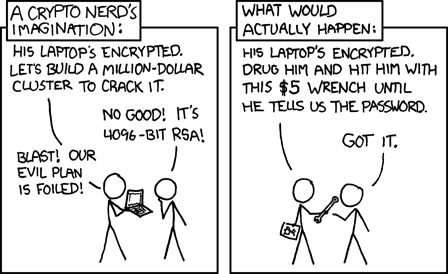
\includegraphics[width=10cm]{pictures_bitmap/security.png}\\
        \url{http://xkcd.com/538/} \href{http://creativecommons.org/licenses/by-nc/2.5/}{ Creative Commons Attribution-NonCommercial 2.5 License}.
\end{center}%
}{}            

\noindent \ldots tout dépends du contexte.


%+++++++++++++++++++++++++++++++++++++++++++++++++++++++++++++++++++++++++++++++++++++++++++++++++++++++++++++++++++++++++++ 
\section{Exemples trigonométriques}
%+++++++++++++++++++++++++++++++++++++++++++++++++++++++++++++++++++++++++++++++++++++++++++++++++++++++++++++++++++++++++++

Nous mettons ici quelque exemples concernant les fonctions trigonométriques, qui n'ont pas pu être mis dans les chapitres le plus adapté, parce que ces derniers sont plus haut dans la table des matière.

\begin{example}[Taylor]     \label{EXooXLYJooKVqhTE}
	Le développement du cosinus est donné par
	\begin{equation}
		\cos(x)=1-\frac{ x^2 }{ 2 }+\frac{ x^4 }{ 4! }-\frac{ x^6 }{ 6! }\cdots
	\end{equation}
	Nous avons donc l'existence d'une fonction $h_1\in o(x^2)$ telle que $\cos(x)=1-\frac{ x^2 }{ 2 }+h_1(x)$. Il existe aussi une autre fonction $h_2\in o(x^4)$ telle que $\cos(x)=1-\frac{ x^2 }{ 2 }+\frac{ x^4 }{ 4! }+h_2(x)$.
\end{example}

\begin{example}[Limite et prolongement par continuité] \label{ExQWHooGddTLE}
    La fonction 
    \begin{equation}
        f(x)=\frac{ \cos(x)-1 }{ x }
    \end{equation}
    n'est pas définie en \( x=0\), mais en la limite
    \begin{equation}
        \lim_{x\to 0} \frac{ \cos(x)-1 }{ x }
    \end{equation}
    nous reconnaissons la limite définissant la dérivée du cosinus en \( 0\), c'est à dire que
    \begin{equation}
        \lim_{x\to 0} \frac{ \cos(x)-1 }{ x }=\sin(0)=0.
    \end{equation}
    Nous avons donc le prolongement par continuité
    \begin{equation}
        \tilde f(x)=\begin{cases}
            \frac{ \cos(x)-1 }{ x }    &   \text{si } x\neq 0\\
            0    &    \text{sinon}.
        \end{cases}
    \end{equation}

    Encore une fois, le graphe de la fonction \(\tilde f\) ne présente aucune particularité autour de \( x=0\).
    \begin{center}
        \input{auto/pictures_tex/Fig_RPNooQXxpZZ.pstricks}
    \end{center}
\end{example}

\begin{example}[Un calcul heuristique de limite]        \label{EXooINLRooPzRWEA}
    Soit à calculer la limite suivante :
    \begin{equation}
        \lim_{x\to 0} \frac{  e^{-2\cos(x)+2}\sin(x) }{ \sqrt{ e^{2\cos(x)+2}}-1 }.
    \end{equation}
    La stratégie que nous allons suivre pour calculer cette limite est de développer certaines parties de l'expression en série de Taylor, afin de simplifier l'expression. La première chose à faire est de remplacer $ e^{y(x)}$ par $1+y(x)$ lorsque $y(x)\to 0$. La limite devient
    \begin{equation}
        \lim_{x\to 0} \frac{ \big( -2\cos(x)+3 \big)\sin(x) }{ \sqrt{-2\cos(x)+2} }.
    \end{equation}
    Nous allons maintenant remplacer $\cos(x)$ par $1$ au numérateur et par $1-x^2/2$ au dénominateur. Pourquoi ? Parce que le cosinus du dénominateur est dans une racine, donc nous nous attendons à ce que le terme de degré deux du cosinus donne un degré un en dehors de la racine, alors que du degré un est exactement ce que nous avons au numérateur : le développement du sinus commence par $x$.

    Nous calculons donc
    \begin{equation}
        \begin{aligned}[]
            \lim_{x\to 0} \frac{ \sin(x) }{ \sqrt{-2\left( 1-\frac{ x^2 }{ 2 } \right)+2} }=\lim_{x\to 0} \frac{ \sin(x) }{ x }=1.
        \end{aligned}
    \end{equation}
    Tout ceci n'est évidement pas très rigoureux, mais en principe vous avez tous les éléments en main pour justifier les étapes.
\end{example}
